% !TeX spellcheck = en_US
%% 字体:方正静蕾简体
%%		 方正粗宋
\documentclass[a4paper,left=1.5cm,right=1.5cm,11pt]{article}
\title{NBA巨星之小皇帝}
\author{周威光整理\footnote{简介:恒天云FTE}}
\date{2017-06-22} 
% 引用宏包
\usepackage[utf8]{inputenc}
\usepackage{fontspec}
\usepackage{cite}
\usepackage{xeCJK}
\usepackage{indentfirst}
\usepackage{titlesec}
\usepackage{etoolbox}%
\makeatletter
\patchcmd{\ttlh@hang}{\parindent\z@}{\parindent\z@\leavevmode}{}{}%
\patchcmd{\ttlh@hang}{\noindent}{}{}{}%
\makeatother

\usepackage{longtable}
\usepackage{empheq}
\usepackage{graphicx}
\usepackage{float}
\usepackage{rotating}
\usepackage{subfigure}
\usepackage{tabu}
\usepackage{amsmath}
\usepackage{setspace}
\usepackage{amsfonts}
\usepackage{appendix}
\usepackage{listings}
\usepackage{xcolor}
\usepackage{geometry}
\setcounter{secnumdepth}{4}
%\titleformat*{\section}{\LARGE}
%\renewcommand\refname{参考文献}
%\titleformat{\chapter}{\centering\bfseries\huge}{}{0.7em}{}{}
\titleformat{\section}{\LARGE\bf}{\thesection}{1em}{}{}
\titleformat{\subsection}{\Large\bfseries}{\thesubsection}{1em}{}{}
\titleformat{\subsubsection}{\large\bfseries}{\thesubsubsection}{1em}{}{}
\renewcommand{\contentsname}{{ \centerline{目{  } 录}}}
\setCJKfamilyfont{cjkhwxk}{STXINGKA.TTF}
%\setCJKfamilyfont{cjkhwxk}{华文行楷}
%\setCJKfamilyfont{cjkfzcs}{方正粗宋简体}
%\newcommand*{\cjkfzcs}{\CJKfamily{cjkfzcs}}
\newcommand*{\cjkhwxk}{\CJKfamily{cjkhwxk}}
%\newfontfamily\wryh{Microsoft YaHei}
%\newfontfamily\hwzs{华文中宋}
%\newfontfamily\hwst{华文宋体}
%\newfontfamily\hwfs{华文仿宋}
%\newfontfamily\jljt{方正静蕾简体}
%\newfontfamily\hwxk{华文行楷}
\newcommand{\verylarge}{\fontsize{60pt}{\baselineskip}\selectfont}  
\newcommand{\chuhao}{\fontsize{44.9pt}{\baselineskip}\selectfont}  
\newcommand{\xiaochu}{\fontsize{38.5pt}{\baselineskip}\selectfont}  
\newcommand{\yihao}{\fontsize{27.8pt}{\baselineskip}\selectfont}  
\newcommand{\xiaoyi}{\fontsize{25.7pt}{\baselineskip}\selectfont}  
\newcommand{\erhao}{\fontsize{23.5pt}{\baselineskip}\selectfont}  
\newcommand{\xiaoerhao}{\fontsize{19.3pt}{\baselineskip}\selectfont} 
\newcommand{\sihao}{\fontsize{14pt}{\baselineskip}\selectfont}      % 字号设置  
\newcommand{\xiaosihao}{\fontsize{12pt}{\baselineskip}\selectfont}  % 字号设置  
\newcommand{\wuhao}{\fontsize{10.5pt}{\baselineskip}\selectfont}    % 字号设置  
\newcommand{\xiaowuhao}{\fontsize{9pt}{\baselineskip}\selectfont}   % 字号设置  
\newcommand{\liuhao}{\fontsize{7.875pt}{\baselineskip}\selectfont}  % 字号设置  
\newcommand{\qihao}{\fontsize{5.25pt}{\baselineskip}\selectfont}    % 字号设置 

\usepackage{diagbox}
\usepackage{multirow}
\boldmath
\XeTeXlinebreaklocale "zh"
\XeTeXlinebreakskip = 0pt plus 1pt minus 0.1pt
\definecolor{cred}{rgb}{0.8,0.8,0.8}
\definecolor{cgreen}{rgb}{0,0.3,0}
\definecolor{cpurple}{rgb}{0.5,0,0.35}
\definecolor{cdocblue}{rgb}{0,0,0.3}
\definecolor{cdark}{rgb}{0.95,1.0,1.0}
\lstset{
	language=bash,
	numbers=left,
	numberstyle=\tiny\color{black},
	showspaces=false,
	showstringspaces=false,
	basicstyle=\scriptsize,
	keywordstyle=\color{purple},
	commentstyle=\itshape\color{cgreen},
	stringstyle=\color{blue},
	frame=lines,
	% escapeinside=``,
	extendedchars=true, 
	xleftmargin=1em,
	xrightmargin=1em, 
	backgroundcolor=\color{cred},
	aboveskip=1em,
	breaklines=true,
	tabsize=4
} 

%\newfontfamily{\consolas}{Consolas}
%\newfontfamily{\monaco}{Monaco}
%\setmonofont[Mapping={}]{Consolas}	%英文引号之类的正常显示,相当于设置英文字体
%\setsansfont{Consolas} %设置英文字体 Monaco, Consolas,  Fantasque Sans Mono
%\setmainfont{Times New Roman}
%\setCJKmainfont{STZHONGS.TTF}
%\setmonofont{Consolas}
% \newfontfamily{\consolas}{YaHeiConsolas.ttf}
\newfontfamily{\monaco}{MONACO.TTF}
\setCJKmainfont{STZHONGS.TTF}
%\setmainfont{MONACO.TTF}
%\setsansfont{MONACO.TTF}
% 自定义添加图片命令
\newcommand{\fic}[1]{\begin{figure}[H]
		\center
		\includegraphics[width=0.8\textwidth]{#1}
	\end{figure}}
	
\newcommand{\sizedfic}[2]{\begin{figure}[H]
		\center
		\includegraphics[width=#1\textwidth]{#2}
	\end{figure}}
% 
\newcommand{\codefile}[1]{\lstinputlisting{#1}}

\newcommand{\interval}{\vspace{0.5em}}

\newcommand{\tablestart}{
	\interval
	\begin{longtable}{p{2cm}p{10cm}}
	\hline}
\newcommand{\tableend}{
	\hline
	\end{longtable}
	\interval}

% 改变段间隔
\setlength{\parskip}{0.2em}
\linespread{1.1}

\usepackage{lastpage}
% 设置页眉页脚
\usepackage{fancyhdr}
\pagestyle{fancy}
\lhead{\space \qquad \space}
\chead{NBA巨星之小皇帝\qquad}
\rhead{\qquad\thepage/\pageref{LastPage}}

% 参考文献
\def\hang{\hangindent\parindent}
\def\textindent#1{\indent\llap{#1\enspace}\ignorespaces}
\def\re{\par\hang\textindent}

\begin{document}
\maketitle
\clearpage
\tableofcontents
\clearpage
\begin{abstract}
勒布朗·詹姆斯(LeBron James),1984年12月30日出生在美国俄亥俄州阿克伦,美国职业篮球运动员,司职小前锋,绰号“小皇帝”,效力于NBA克利夫兰骑士队。
勒布朗·詹姆斯在2003年NBA选秀中于首轮第1顺位被克利夫兰骑士队选中。2003-2010年,詹姆斯效力于骑士队,期间2次当选NBA最有价值球员(MVP)。
2010年,詹姆斯转会至迈阿密热火队,与德怀恩·韦德以及克里斯·波什组成“三巨头”阵容。2012年,詹姆斯得到NBA个人生涯的第3座常规赛MVP,第1个总冠军和总决赛MVP。
詹姆斯代表美国男篮获得了2012年伦敦奥运会金牌,追平了迈克尔·乔丹在1992年所创的纪录。2013年,詹姆斯获得第4个常规赛MVP、第2个NBA总冠军和第2个总决赛MVP,实现两连冠。
2014年,詹姆斯回归骑士,与凯里·欧文、凯文·乐福组成“三巨头”阵容。2016年,詹姆斯带领骑士逆转战胜卫冕冠军勇士获得队史首个总冠军和个人第3个总决赛MVP。
2017年06月12日,美国《福布斯》杂志公布了2017年度全球百位名人榜,美国篮球运动员勒布朗·詹姆斯(8600万美元)排名第十。
\end{abstract}
\bf{关键词:}\it{小皇帝},\it{MVP},\it{三巨头},\it{天选之子} 
\clearpage
 
\section{一级标题}
\subsection{二级标题}
\subsubsection{三级标题}
\begin{itemize}
	\item[1.]小标题 
	\sizedfic{0.4}{king.jpg}
	\begin{center}
	小皇帝
	\end{center}
	\begin{figure}[h!]
	\centering
	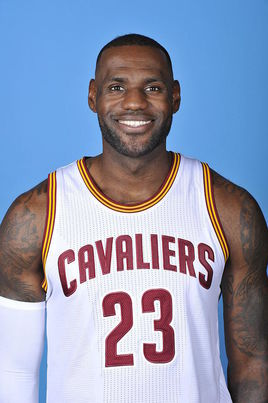
\includegraphics[scale=1.7]{king.jpg}
	\caption{The Universe}
	\label{fig:univerise}
	\end{figure}
	\begin{itemize}
		\item[(1).] 第一大象
		\item[(2).] 第二大象
		\begin{itemize}
			\item[1).] 第一小巷
			\item[2).] 第二小想
		\end{itemize}
	\end{itemize}
\end{itemize}
常规赛场均数据
\begin{tabular}[c]{|l|l|l|}
\hline
\hline
赛季 & 球队 & 出场\\
\hline\hline
2005-06 & 骑士 & 13\\
2005-06 & 骑士 & 13\\
\hline
\end{tabular}
常规赛场均数据\\
\section{你好中国}
中国在East Asia.
\subsection{Hello Beijing}
北京是capital of China.
\subsubsection{Hello Dongcheng District}
\paragraph{Tian'anmen Square}
is in the center of Beijing
\subparagraph{Chairman Mao}
is in the center of 天安门广场。
\subsection{Hello 山东}
\paragraph{山东大学} is one of the best university in 山东。\\\\
\begin{center}
\begin{tabular}{|l|c|r|}
 \hline
操作系统& 发行版& 编辑器\\
 \hline
Windows & MikTeX & TexMakerX \\
 \hline
Unix/Linux & teTeX & Kile \\
 \hline
Mac OS & MacTeX & TeXShop \\
 \hline
通用& TeX Live & TeXworks \\
 \hline
\end{tabular}
\end{center}
\begin{lstlisting}
代码块
\end{lstlisting}
天安门广场天安门广场天安门广场天安门广场天安门广场天安门广场天安门广场天安门\par
广场天安门广场天安门广场天安门广场天安门广场天安门广场天安门广场
天安门广场天安门广场天安门广场天安门广场天安门广场天安门广场天安门广场天安门广场天安\par
门广场天安门广场天安门广场天安门广场天安门广场天安门广场
天安门广场天安门广场天安门广场天安门广场天安门广场天安门广场天安门广场天安门广场天安门广场天安门广场天安门广场
天安门广场天安门广场天安门广场天安门广场天安门广场天安门广场天安门广场天安门广场天安门广场天安门广场天安门广场


\re{[1]} Nordhaus E,Stewart B,WhiteA.On the Maximum Genus of a Graph.{\it J.combinatorial Theory B},1971,11:258-267  
\re{[2]} Skoviera M.The Maximum Genus of Graphs of Diameter Two.{\it Discrete Math}.1991, 87:175-180
\end{document}